\chapter{Arhitektura i dizajn sustava}
		
		Arhitektura se može podijeliti na tri podsustava:
		\begin{itemize}
			\item 	\textit{Web aplikacija}
			\item 	\textit{Web poslužitelj}  
			\item 	\textit{Baza podataka}
		\end{itemize}
	
		\textit{\textbf{Web preglednik}} je program koji korisniku omogućuje pregled web-stranica. Svaki internetski  preglednik  je  u suštini prevoditelj, on interpretira programski jezik kojim je stranica napisana te korisniku prikazuje rezultat tog prevođenja. Korisnik  putem  web  preglednika šalje  zahtjev  web poslužitelju.
		
		\textit{\textbf{Web poslužitelj}} je osnova rada web aplikacije. Njegova primarna zadaća je komunikacija klijenta s aplikacijom koja se odvija preko HTTP (engl.HyperText Transfer Protocol) protokola, što je standardni protokol u prijenosu informacija na webu. Poslužitelj je onaj koji pokreće web aplikaciju te joj prosljeđuje zahtjev.
		
		Korisnik koristi web aplikaciju za obrađivanje željenih zahtjeva. Web aplikacija obrađuje zahtjev te, ovisno o zahtjevu, pristupa bazi podataka, nakon čega preko poslužitelja vraća odgovor korisniku, u obliku HTML dokumenta vidljivog u web pregledniku.
		
		Naša web aplikacija je podijeljena na dva glavna dijela: \textit{backend} i \textit{frontend}. Za rad na backendu odlučili smo se za programski jezik Java. Koristimo radni okvir Spring Boot. Java Spring Boot nam nudi unaprijed konfigurirane klase Spring radnog okvira, što nam štedi puno vremena jer se ne moramo zamarati konfiguracijom.\\ \\
		Backend je podijeljen u tri sloja: \textit{controller}, \textit{service} i \textit{repository}. \\ \\
		\begin{figure}[H]
				\centering
				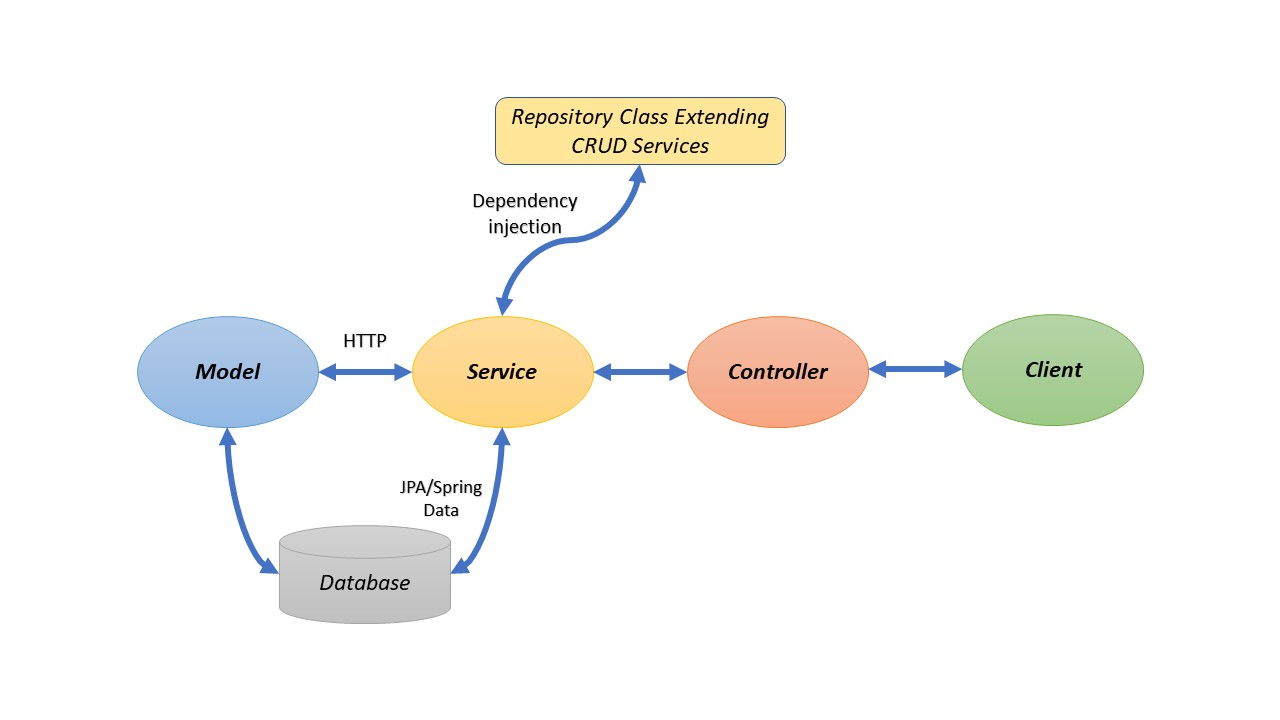
\includegraphics[width=0.9\textwidth]{slike/Spring_dijagram.jpg}
				\caption{Spring dijagram}
				\label{fig:mesh1}
		\end{figure}

		\begin{itemize}
			\item 	\textit{\textit{\textbf{Controller}} komunicira s frontendom  te obrađuje HTTP zahtjeve koje mu frontend pošalje te je u skladu s REST principima.}
			\item 	\textit{\textbf{Service}} sadrži poslovnu logiku aplikacije te je veza između \textit{controllera} i \textit{repositoryja}. On prima podatke iz \textit{controllera} i \textit{repositoryja} te odlučuje što će s tim podacima napraviti (odbaciti, proslijediti, izmijeniti,...) 
			\item 	\textit{\textbf{Repository}} komunicira s bazom podataka te sve zahtjeve prima od servisa i njemu ih vraća.
		\end{itemize}
	
			Uz to koristimo još \textit{entitete} i \textit{DTOs (Data transfer objects)}. DTO je objekt koji se prenosi između procesa. On ne sadrži nikakvu poslovnu logiku, ali može sadržavati mehanizme serijalizacije i deserijalizacije za prijenos podataka.\\ 

			Za rad na frontendu smo se odlučili za \textit{React (JavaScript library)}. Reactov kod se sastoji od entiteta i komponenti. Komponente mogu biti  prikazane u određenom elementu u DOM-u. React je odličan jer se mogu kreirati komponente koje možemo ponovno upotrijebiti bez da pišemo isti/sličan kod na više mjesta.\\
			Razvojno okruženje koje koristimo je InteliJ.

				
		\section{Baza podataka}
			
			Za potrebe naše aplikacije koristit ćemo relacijsku bazu podataka. Baza podataka
			se sastoji od više relacija (takozvanih tablica ili entiteta). Svaka od tih relacija je definirana imenom relacije i skupom atributa koji pobliže opisuju samu relaciju.
			Baza podataka nam služi za pohranu, izmjenu i dohvat potrebnih podataka. Baza
			podataka ove aplikacije sastoji se od sljedećih entiteta:
			\begin{itemize}
				\item 	\textbf{Korisnik}
				\item 	\textbf{Izlet}
				\item 	\textbf{Planinarski dom}
				\item 	\textbf{Geografsko područje}
				\item 	\textbf{Ocjena}
			\end{itemize}
				
		
		
			\subsection{Opis tablica}
			

				\textbf{Korisnik:} Ovaj entitet sadržava sve relevantne informacije o korisniku aplikacije.
				Sadrži sljedeće atribute: jedinstveni identifikator, korisničko ime, lozinku,
				ime, prezime, link za sliku profila, razinu ovlasti korisnika. Ovaj entitet
				je u vezi: \textit{Many-to-Many} s entitetom \textit{Izlet} preko atributa \textit{ID}. Primarni ključ
				entiteta jest atribut \textit{ID}.
				
				\begin{longtabu} to \textwidth {|X[7, l]|X[6, l]|X[21, l]|}
					
					\hline \multicolumn{3}{|c|}{\textbf{Korisnik}}	 \\[3pt] \hline
					\endfirsthead
					
					\hline \multicolumn{3}{|c|}{\textbf{Korisnik}}	 \\[3pt] \hline
					\endhead
					
					\hline 
					\endlastfoot
					
					\cellcolor{LightGreen}ID & BIGINT	&  Jedinstveni identifikator korisnika 	\\ \hline
					Korisničko ime & VARCHAR & Korisničko ime  	\\ \hline 
					Lozinka & VARCHAR & Hash lozinke		\\ \hline 
					Ime & VARCHAR	&  	Ime korisnika			\\ \hline 
					Prezime & VARCHAR	& Prezime korisnika			\\ \hline 
					Slika profila & VARCHAR	&Link za sliku profila		\\ \hline 
					Razina ovlasti& VARCHAR	& Korisnikova uloga		\\ \hline 
			
				\end{longtabu}
			
				\textbf{Izlet:} Ovaj entitet sadržava sve relevantne informacije za jedan izlet.
				Sadrži sljedeće atribute: jedinstveni identifikator, vrh, trajanje, duljinu staze, težinu,
				oznaku o tome je li privatan ili javan i identifikator za ocjenu. Ovaj entitet
				je u vezi: \textit{Many-to-Many} s entitetom \textit{Korisnik} preko atributa \textit{ID}, \textit{Many-to-Many} s entitetom \textit{Planinarski dom} preko atributa \textit{ID},   \textit{Many-to-One} s entitetom \textit{Geografsko područje} preko atributa \textit{ID} i \textit{One-to-Many} s entitetom \textit{Ocjena} preko atributa \textit{ID} . Primarni ključ entiteta jest atribut \textit{ID}.
				
				\begin{longtabu} to \textwidth {|X[7, l]|X[6, l]|X[21, l]|}
					
					\hline \multicolumn{3}{|c|}{\textbf{Izlet}}	 \\[3pt] \hline
					\endfirsthead
					
					\hline \multicolumn{3}{|c|}{\textbf{Izlet}}	 \\[3pt] \hline
					\endhead
					
					\hline 
					\endlastfoot
					
					\cellcolor{LightGreen}ID & BIGINT	&  Jedinstveni identifikator izleta 	\\ \hline
					Vrh				& VARCHAR 	& Naziv vrha izleta  	\\ \hline 
					Trajanje		& BIGINT 	& Vrijeme trajanja izleta		\\ \hline 
					Duljina 		& DECIMAL	& Duljina staze			\\ \hline 
					Težina 			& BIGINT	& Težina staze			\\ \hline 
					Javan			& BOOLEAN	& Oznaka je li izlet javan ili privatan		\\ \hline 
					Ocjena ID		& BIGINT	& Strani ključ koji povezuje relaciju \textit{Izlet}	i \textit{Ocjena}	\\ \hline 
					Područje ID		& BIGINT	& Strani ključ koji povezuje relaciju \textit{Izlet}	i \textit{Geografsko područje}	\\ \hline 
					Opis			& VARCHAR	& Kratki opis izleta		\\ \hline 
					
				\end{longtabu}
			
			
				\textbf{Planinarski dom:} Ovaj entitet sadržava sve relevantne informacije o planinarskom domu.
				Sadrži sljedeće atribute: jedinstveni identifikator, naziv doma, oznaka o prenoćištu, oznaka o hrani, oznaka o vodi i oznaka o struji. Ovaj entitet
				je u vezi: \textit{Many-to-Many} s entitetom \textit{Izlet} preko atributa \textit{ID}, Primarni ključ entiteta jest atribut \textit{ID}.
				
				
				\begin{longtabu} to \textwidth {|X[7, l]|X[6, l]|X[21, l]|}
					
					\hline \multicolumn{3}{|c|}{\textbf{Planinarski dom}}	 \\[3pt] \hline
					\endfirsthead
					
					\hline \multicolumn{3}{|c|}{\textbf{Planinarski dom}}	 \\[3pt] \hline
					\endhead
					
					\hline 
					\endlastfoot
					
					\cellcolor{LightGreen}ID & BIGINT	&  Jedinstveni identifikator planinarskog doma 	\\ \hline
					Naziv			& VARCHAR 	& Naziv planinarskog doma  	\\ \hline 
					Noćenje			& BOOLEAN 	& Oznaka o prenoćištu		\\ \hline 
					Hrana 			& BOOLEAN	& Oznaka o opskrbi hranom			\\ \hline 
					Voda 			& BOOLEAN	& Oznaka o opskrbi vodom			\\ \hline 
					Struja			& BOOLEAN	& Oznaka o dostupnosti struje		\\ \hline 
					
					
				\end{longtabu}
			
			
				\textbf{Geografsko područje:} Ovaj entitet sadržava sve relevantne informacije o geografskom području.
				Sadrži sljedeće atribute: jedinstveni identifikator, naziv područja. Ovaj entitet
				je u vezi: \textit{Many-to-Many} s entitetom \textit{Izlet} preko atributa \textit{ID}, Primarni ključ entiteta jest atribut \textit{ID}.
				
				
				\begin{longtabu} to \textwidth {|X[7, l]|X[6, l]|X[21, l]|}
					
					\hline \multicolumn{3}{|c|}{\textbf{Geografsko područje}}	 \\[3pt] \hline
					\endfirsthead
					
				
					
					\hline 
					\endlastfoot
					
					\cellcolor{LightGreen}ID & BIGINT	&  Jedinstveni identifikator geografskog područja 	\\ \hline
					Naziv			& VARCHAR 	& Naziv geografskog područja 	\\ \hline 
				
					
					
				\end{longtabu}
			
					
				\textbf{Ocjena:} Ovaj entitet sadržava sve relevantne informacije o ocjeni. Sadrži sljedeće atribute: jedinstveni identifikator, ocjena i komentar. Ovaj entitet
				je u vezi: \textit{Many-to-One} s entitetom \textit{Izlet} preko atributa \textit{ID}, Primarni ključ entiteta jest atribut \textit{ID}.
				
				
				\begin{longtabu} to \textwidth {|X[7, l]|X[6, l]|X[21, l]|}
					
					\hline \multicolumn{3}{|c|}{\textbf{Ocjena}}	 \\[3pt] \hline
					\endfirsthead
					
					\hline \multicolumn{3}{|c|}{\textbf{Ocjena}}	 \\[3pt] \hline
					\endhead
					
					\hline 
					\endlastfoot
					
					\cellcolor{LightGreen}ID & BIGINT	&  Jedinstveni identifikator geografskog područja 	\\ \hline
					Ocjena					& BIGINT 	& Predstavlja ocjenu izleta 	\\ \hline 
					Komentar				& VARCHAR 	& Komentar uz ocjenu	\\ \hline 
					
					
				\end{longtabu}
				
			
			
			
			
			
			
			
			
			
			
			
			
			
			
			
			
			
			
			
			
			
			
			
			\subsection{Dijagram baze podataka}
				\begin{figure}[H]
				\centering
				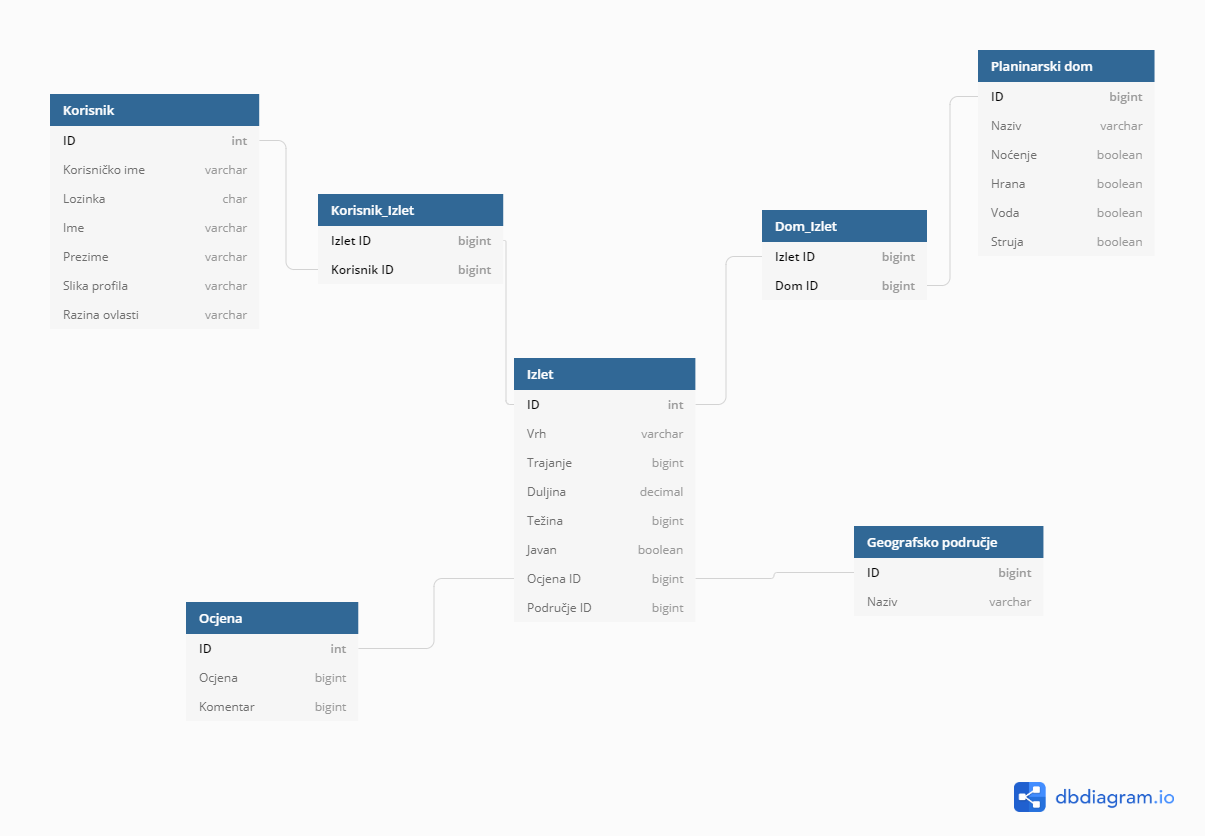
\includegraphics[width=1.1\textwidth]{slike/Baza_dijagram.png}
				\caption{Dijagram baze podataka}
				\label{fig:mesh1}
			\end{figure}
			\eject
			
			
		\section{Dijagram razreda}
			Na slikama: (4.3, 4.4 i 4.5) nalaze se dijagrami razreda. Na dijagramima se nalaze komponente koje opisuju trenutno stanje aplikacije, ali i konceptualni prikaz komponenti koje će se tek pojaviti (npr. \textit{Event, Badge, Administrator...}). U daljnjem radu i razvoju aplikacije doći će do promjena i nadopuna dijagrama razreda. \\
			Dijagrami su podijeljeni u tri cjeline (\textit{Controller, DTO} i \textit{Model}) radi lakšeg snalaženja i preglednosti.
			
			\begin{figure}[H]
				\centering
				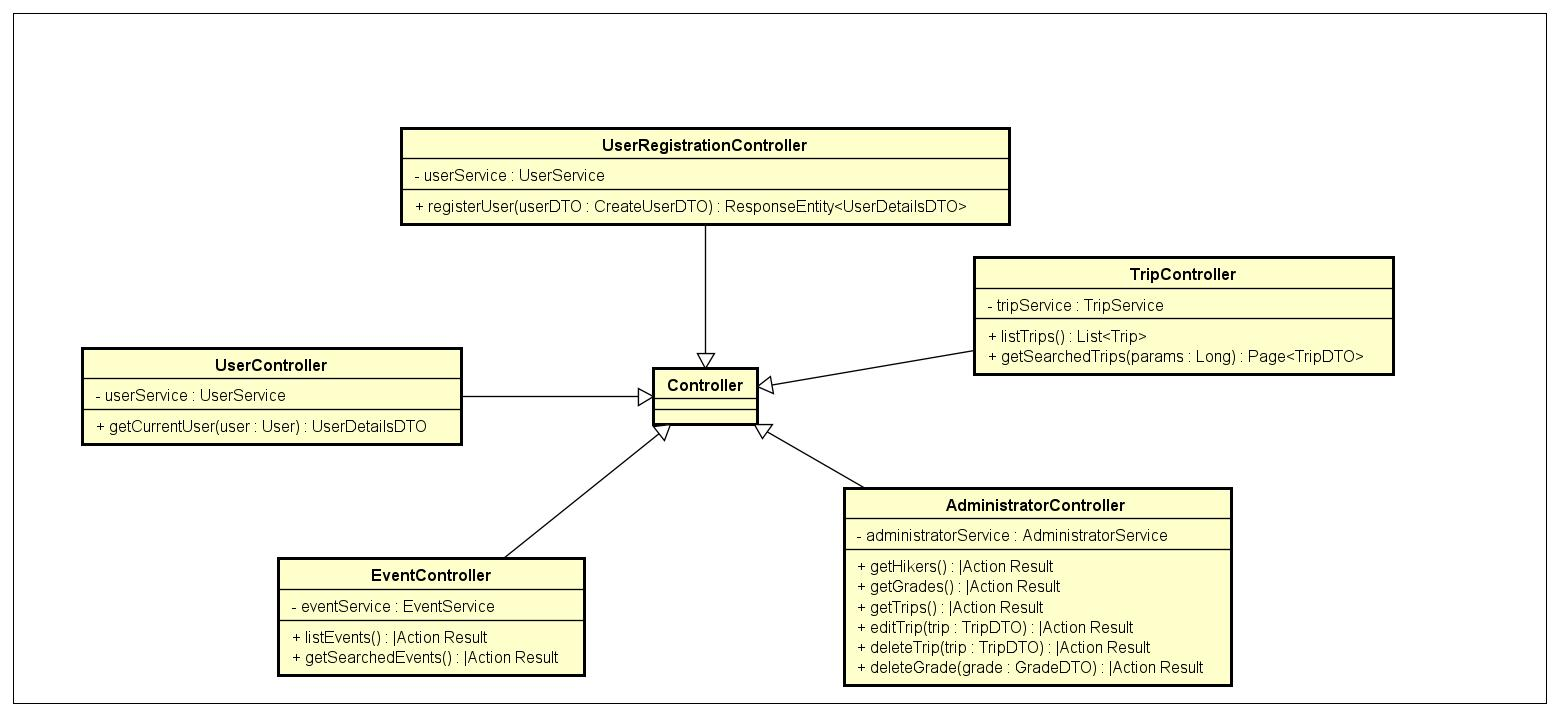
\includegraphics[width=1.1\textwidth]{slike/Controller_dijagram.jpg}
				\caption{Dijagram razreda Controller}
				\label{fig:mesh1}
			\end{figure} 
			
			\begin{figure}[H]
				\centering
				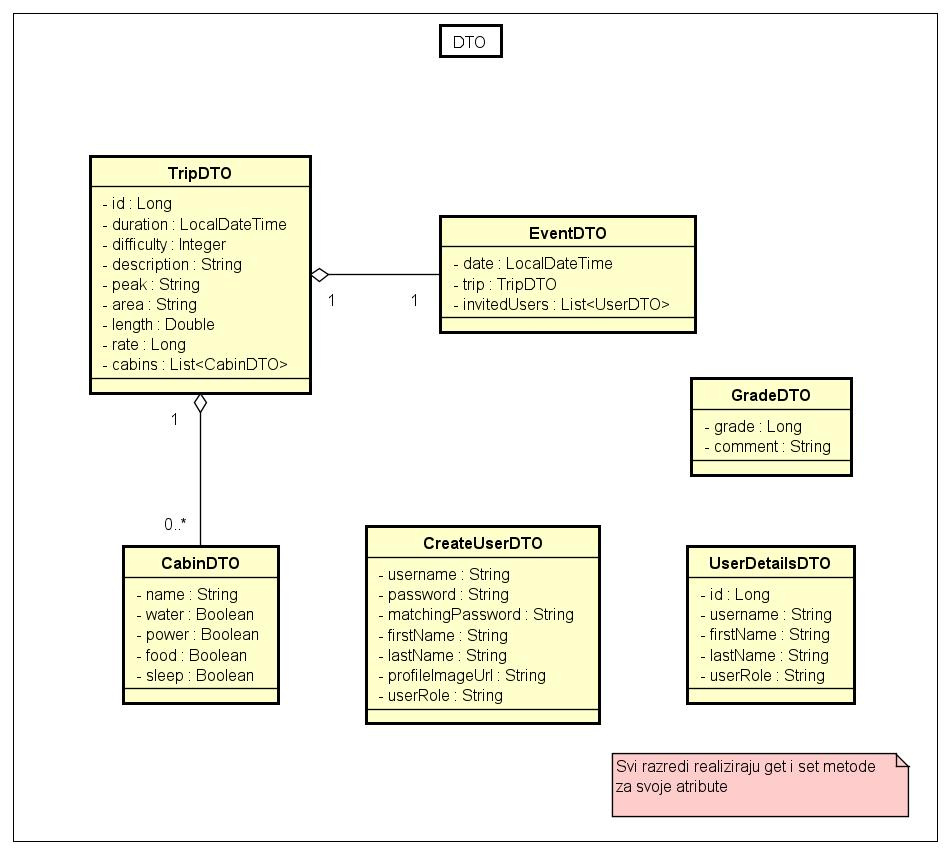
\includegraphics[width=0.9\textwidth]{slike/DTO_dijagram.jpg}
				\caption{Dijagram razreda DTO}
				\label{fig:mesh1}
			\end{figure}
			
			\begin{figure}[H]
				\centering
				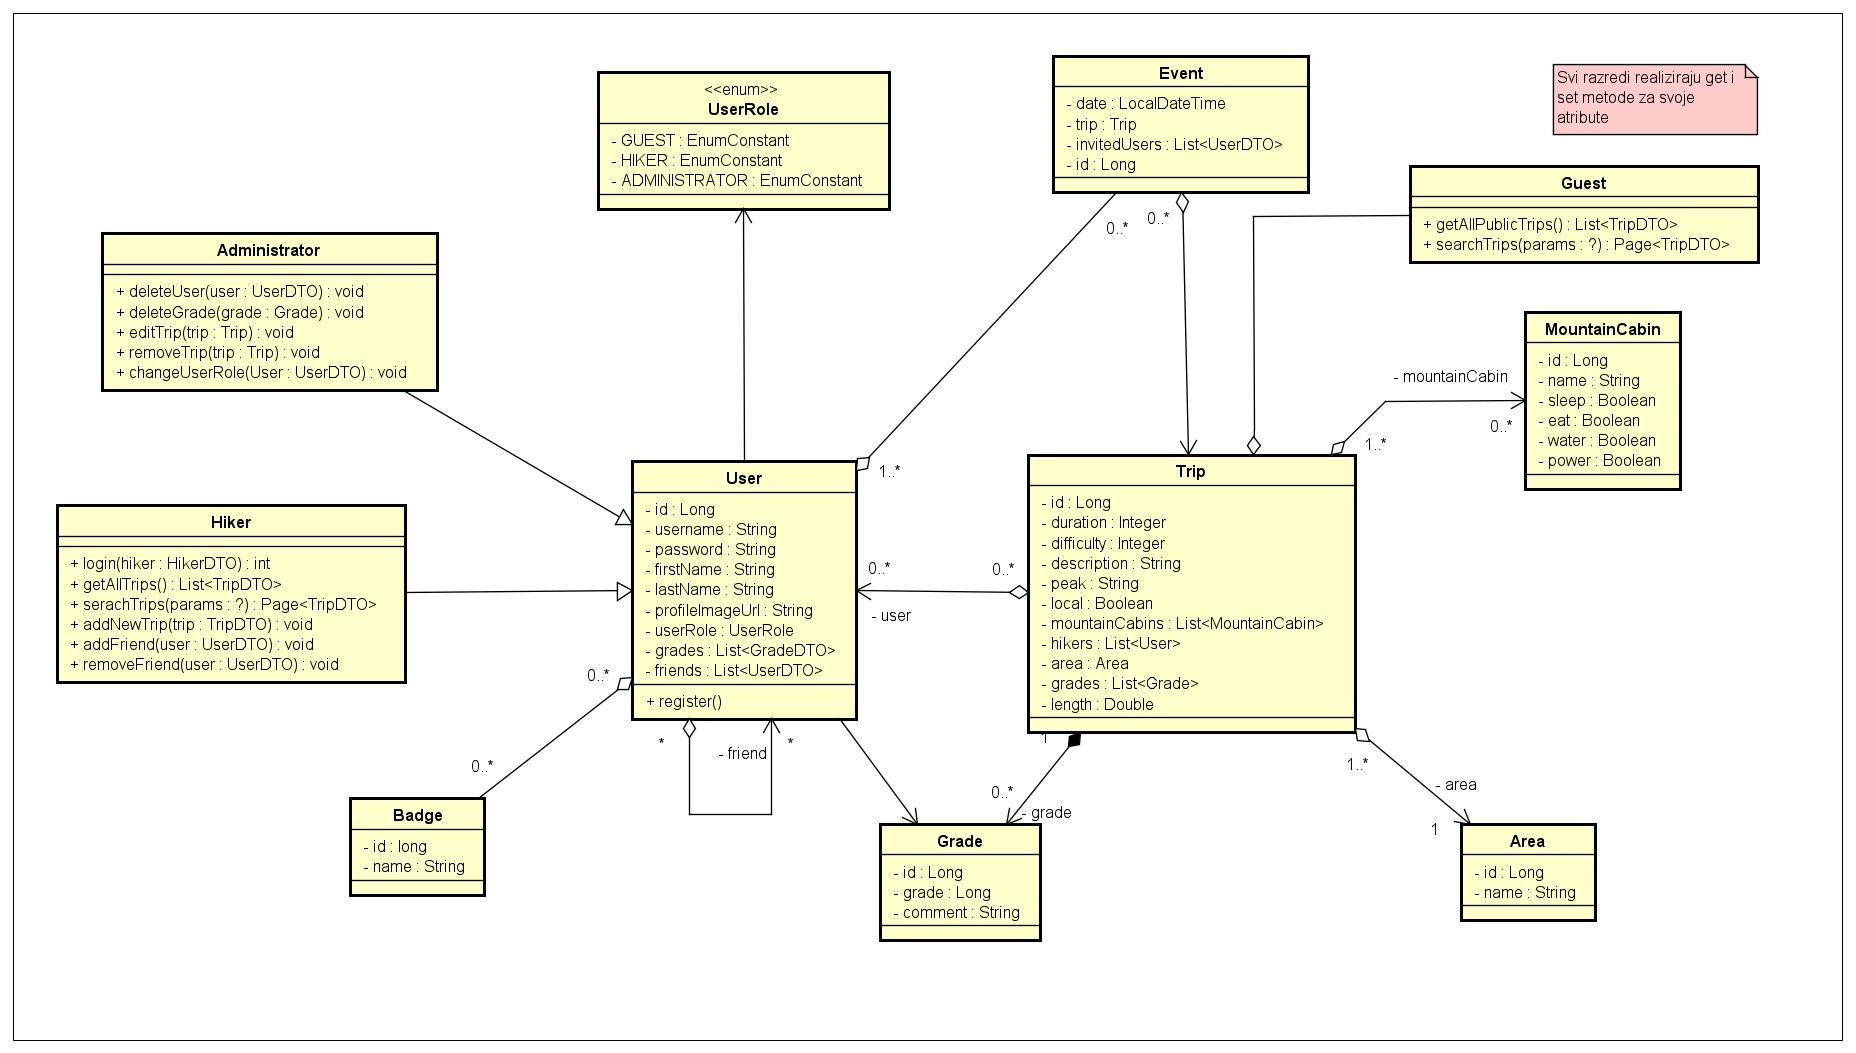
\includegraphics[width=0.9\textwidth]{slike/Model_dijagram.jpg}
				\caption{Dijagram razreda Model}
				\label{fig:mesh1}
			\end{figure} 
			
			\textit{Potrebno je priložiti dijagram razreda s pripadajućim opisom. Zbog preglednosti je moguće dijagram razlomiti na više njih, ali moraju biti grupirani prema sličnim razinama apstrakcije i srodnim funkcionalnostima.}\\
			
			\textbf{\textit{dio 1. revizije}}\\
			
			\textit{Prilikom prve predaje projekta, potrebno je priložiti potpuno razrađen dijagram razreda vezan uz \textbf{generičku funkcionalnost} sustava. Ostale funkcionalnosti trebaju biti idejno razrađene u dijagramu sa sljedećim komponentama: nazivi razreda, nazivi metoda i vrste pristupa metodama (npr. javni, zaštićeni), nazivi atributa razreda, veze i odnosi između razreda.}\\
			
			\textbf{\textit{dio 2. revizije}}\\			
			
			\textit{Prilikom druge predaje projekta dijagram razreda i opisi moraju odgovarati stvarnom stanju implementacije}
			
			
			
			\eject
		
		\section{Dijagram stanja}
			
			
			\textbf{\textit{dio 2. revizije}}\\
			
			\textit{Potrebno je priložiti dijagram stanja i opisati ga. Dovoljan je jedan dijagram stanja koji prikazuje \textbf{značajan dio funkcionalnosti} sustava. Na primjer, stanja korisničkog sučelja i tijek korištenja neke ključne funkcionalnosti jesu značajan dio sustava, a registracija i prijava nisu. }
			
			
			\eject 
		
		\section{Dijagram aktivnosti}
			
			\textbf{\textit{dio 2. revizije}}\\
			
			 \textit{Potrebno je priložiti dijagram aktivnosti s pripadajućim opisom. Dijagram aktivnosti treba prikazivati značajan dio sustava.}
			
			\eject
		\section{Dijagram komponenti}
		
			\textbf{\textit{dio 2. revizije}}\\
		
			 \textit{Potrebno je priložiti dijagram komponenti s pripadajućim opisom. Dijagram komponenti treba prikazivati strukturu cijele aplikacije.}